\documentclass[paper=a4, fontsize=11pt]{scrartcl}

\usepackage[T1]{fontenc} % Use 8-bit encoding that has 256 glyphs
\usepackage[english]{babel} % English language/hyphenation
\usepackage{amsmath,amsfonts,amsthm,pst-plot,a4wide} % Math packages
\usepackage{epsfig,graphics}
\usepackage{tikz}

\usepackage{fancyhdr} % Custom headers and footers
\pagestyle{fancyplain} % Makes all pages in the document conform to the custom headers and footers
\fancyhead{} % No page header - if you want one, create it in the same way as the footers below
\fancyhead[L]{CSI3109, AUTOMATA AND FORMAL LANGUAGES}
\fancyhead[R]{{\textit{Yo-Sub Han}}}
\fancyfoot[L]{} % Empty left footer
\fancyfoot[C]{} % Empty center footer
\fancyfoot[R]{\thepage~~of~~\pageref{lastpage}} 
%\renewcommand{\headrulewidth}{0pt} % Remove header underlines
\renewcommand{\footrulewidth}{0pt} % Remove footer underlines
\setlength{\headheight}{13.6pt} % Customize the height of the header
\setlength\parindent{0pt} 
\newcommand{\horrule}[1]{\rule{\linewidth}{#1}} % Create horizontal rule command with 1 argument of height


\begin{document}
\begin{center}
YONSEI UNIVERSITY\\
Department of Computer Science\\[0.1in]
{\textbf {CSI3109 Automata and Formal Languages, SPRING 2017}} \\[0.1in]
{\large{\textbf{Homework No.2}}}\\[0.1in]
{\textbf{DUE:}} 2017.04.17 13:00:00pm
\end{center}


\vspace{0.1in}
\noindent
{\textbf{Student ID:}} 2014117007 \\[0.15in]
{\textbf{Student Name:}} Chung, Ji-Wan
\vspace{0.3in}

%----------------------------------------------------------------------
% Yon don't need to change anything except for your ID and name above
%----------------------------------------------------------------------


\begin{enumerate}
\item 
Given a DFA~$A=(Q, \Sigma, \delta, s, F)$, where
$$Q = \{1,2,3,4,5,6\}, \Sigma = \{a,b\}, s = 1, F = \{2,5,6\}$$ and
$\delta$
is defined as follows:
\begin{center}
\begin{tabular}{ l || c | c }
 & $a$ & $b$\\
\hline \hline
1 & 2 & 3\\
2 & 2 & 4\\
3 & 4 & 5\\
4 & 2 & 6\\
5 & 5 & 4\\
6 & 6 & 6
\end{tabular}
\end{center}

Run the TF~(Table Filling) algorithm and  draw a minimal DFA
for $L(A)$.

\vspace{1cm}
\[
  \begin{bmatrix}
    2 & X & - & - & - & - \\
    3 & X & X & - & - & - \\
    4 & X & X & X & - & - \\
    5 & X &  & X & X & - \\
    6 & X & X & X & X & X \\
     / & 1 & 2 & 3 & 4 & 5 
  \end{bmatrix}
\]
Equivalence Class = $(1), (3), (4), (6), (2,5)$

\vspace{1cm}
\textit{$\rightarrow$ drawing on the next page}

\newpage

\begin{center}
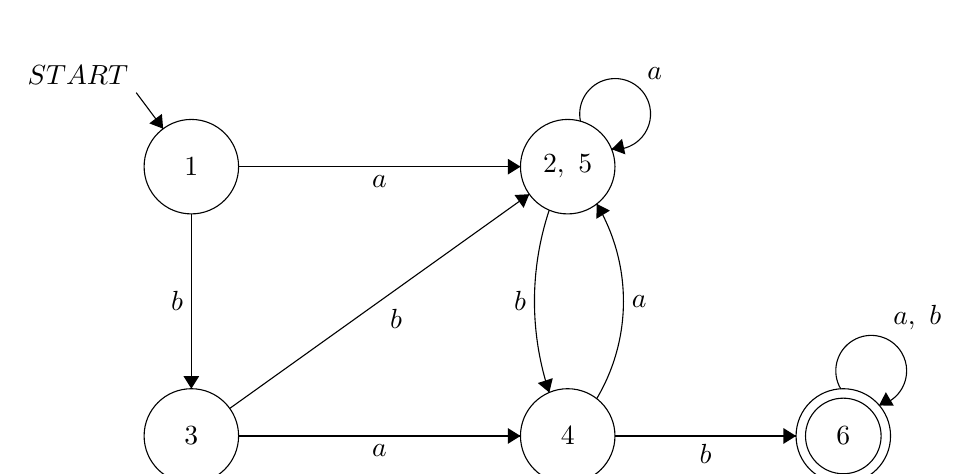
\begin{tikzpicture}[scale=0.2]
\tikzstyle{every node}+=[inner sep=0pt]
\draw [black] (12.9,-26.6) circle (3);
\draw (12.9,-26.6) node {$1$};
\draw [black] (12.9,-43.7) circle (3);
\draw (12.9,-43.7) node {$3$};
\draw [black] (36.8,-26.6) circle (3);
\draw (36.8,-26.6) node {$2,\mbox{ }5$};
\draw [black] (36.8,-43.7) circle (3);
\draw (36.8,-43.7) node {$4$};
\draw [black] (54.3,-43.7) circle (3);
\draw (54.3,-43.7) node {$6$};
\draw [black] (54.3,-43.7) circle (2.4);
\draw [black] (9.4,-21.9) -- (11.11,-24.19);
\draw (5.7,-21.4) node [above] {$START$};
\fill [black] (11.11,-24.19) -- (11.03,-23.25) -- (10.23,-23.85);
\draw [black] (15.9,-26.6) -- (33.8,-26.6);
\fill [black] (33.8,-26.6) -- (33,-26.1) -- (33,-27.1);
\draw (24.85,-27.1) node [below] {$a$};
\draw [black] (12.9,-29.6) -- (12.9,-40.7);
\fill [black] (12.9,-40.7) -- (13.4,-39.9) -- (12.4,-39.9);
\draw (12.4,-35.15) node [left] {$b$};
\draw [black] (15.9,-43.7) -- (33.8,-43.7);
\fill [black] (33.8,-43.7) -- (33,-43.2) -- (33,-44.2);
\draw (24.85,-44.2) node [below] {$a$};
\draw [black] (15.34,-41.95) -- (34.36,-28.35);
\fill [black] (34.36,-28.35) -- (33.42,-28.4) -- (34,-29.22);
\draw (25.9,-35.65) node [below] {$b$};
\draw [black] (37.61,-23.723) arc (192.01279:-95.98721:2.25);
\draw (42.33,-21.09) node [above] {$a$};
\fill [black] (39.58,-25.49) -- (40.46,-25.82) -- (40.25,-24.84);
\draw [black] (35.625,-40.943) arc (-161.60194:-198.39806:18.355);
\fill [black] (35.63,-40.94) -- (35.85,-40.03) -- (34.9,-40.34);
\draw (34.19,-35.15) node [left] {$b$};
\draw [black] (38.637,-28.962) arc (30.75886:-30.75886:12.099);
\fill [black] (38.64,-28.96) -- (38.62,-29.91) -- (39.48,-29.39);
\draw (40.84,-35.15) node [right] {$a$};
\draw [black] (39.8,-43.7) -- (51.3,-43.7);
\fill [black] (51.3,-43.7) -- (50.5,-43.2) -- (50.5,-44.2);
\draw (45.55,-44.2) node [below] {$b$};
\draw [black] (54.14,-40.716) arc (210.80141:-77.19859:2.25);
\draw (59,-36.97) node [above] {$a,\mbox{ }b$};
\fill [black] (56.57,-41.76) -- (57.51,-41.78) -- (57,-40.92);
\end{tikzpicture}
\end{center}

\newpage

\item Prove that the following languages are not regular. You may use
the
pumping lemma or the closure properties of regular languages under
union, intersection and complement.
\begin{enumerate}
\item $L = \{0^n1^m0^n \mid m, n \ge 0\}$.

\vspace{1cm}
\textbf{Answer:}
	\begin{enumerate}
		\item Assume that $L$ is regular. Then, there is a pumping constant $n\ge1$ strings with length
			greater than or equal to n can be 'pumped' according to pumping lemma.
		\item For an arbitrary natural number $l\ge n$, we take a string $w = 0^l1^l0^l\in L$.
		\item Following pumping lemma, since $|w|> l \ge n$ $w$ can be divided into $w=xyz$ of which
			$|xy|\le n \le l$ and  $|y| > 0$ holds.
		\item Since $|xy| \le l$, we can safely deduct the substrings $x, y$ are composed of the symbol 				$0$ only. Likewise we define $x=0^i, y=0^{j-i}$ for some $0 \le i < j \le n \le l$.
		\item Then we consider another string $w'=xy^2z=0^i0^{2(j-i)}0^{l-j}1^l0^l=0^{l+(j-i)}1^l0^l$ which
			can be pumped from $w$. Since $|y| > 0$, $j-i >0$. Then $l + (j-i) > l$, rendering $w' \notin 
			L$. For that contradicts our assumption that the pumping lemma holds for $L$, $L$ is not 				regular.
	\end{enumerate}
\newpage

\item $L = \{w  \mid w \in \{0, 1\}^* \textrm{~is not a
palindrome}\}$.\\
(A palindrome is a string that reads the same forward and backward.
e.g.: racecar)

\vspace{1cm}
\textbf{Answer:}
	\begin{enumerate}
		\item Assume $L$ is regular. Then, $P = \overline{L} = \{w|w \in \{0,1\}^* \text{is a palindrome} \}$ is also
			regular since a regular language is closed under complement.
		\item We take contrapositive of $i)$. Then, if we can prove the nonregularity of $P$ we prove 
			the nonregularity of $L$ automatically.
		\item Now, define a Language $L'=L(0^*1^*0^*)$. We can see $L'$ is regular by its defition relying on 				a regular expression. Then we recognize $L'\cap P$ equals the language of $a)$, which is 				already proven unregular. If $P$ is regular, the language of $a)$ should be regular since a
			regular language is closed under intersection, which is not the case. So $P$ is nonregular.
		\item Combining $ii)$and $iii)$, we can deduct $L$ is also a nonregular language.
	\end{enumerate}
\end{enumerate}

\newpage


\item Show that the regular languages are closed under the
following operations:
\begin{enumerate}
\item 
$$
\mathbb{DROPOUT}(L) = \{ xz \mid xyz \in L, \textrm{~where~} x,z \in
\Sigma^*, y \in \Sigma \}.
$$
Namely, $\mathbb{DROPOUT}(L)$ is the language containing all strings
that can be obtained by removing one symbol from a string in $L$.\\
For example, if $L = \{012\}$, then $\mathbb{DROPOUT}(L) = \{12, 02,
01\}$.

\vspace{1cm}
\textbf{Answer:}
\begin{enumerate}
		\item If $L$ is regular, there is at least one corresponding regular expression $E$ recognizing
			$L$.
		\item Now we construct a regular expression $E'$ recognizing the language of 							$\mathbb{DROPOUT}(L)$. Beforehand, we define a function $f$ which accepts a RegEx $E''$
			and returns a set formed by processing $\mathbb{DROPOUT}$ on the language accepted
			by that expression.
		\item For $E'' = \emptyset$, $f(\emptyset) = \emptyset$ by definition.
		\item For $E'' = \{ \epsilon \}$, $f( \{ \epsilon \}) = \emptyset$ by definition.
		\item For $E'' = \{\sigma\}$, $f(\{\sigma\}) = \{ \epsilon \}$ by definition.
		\item For union operation, $f(E_1 + E_2) = f(L(E_1) \cup L(E_2))$. Note that for a string $w$, $w \in         L(E_1) \cup L(E_2)$ implies either $w \in L(E_1)$ or $w \in L(E_2)$ holds. For the former, $f(\{w\}) \subset f(L(E_1))$ and $f(L(E_1) \cup L(E_2))$ respectively. For the latter, $f(\{w\}) \subset f(L(E_2))$ and $f(L(E_1) \cup L(E_2))$. So every $w$ is in $f(L(E_1) \cup L(E_2))$ if and only if it is in $f(L(E_1)) \cup f(L(E_2))$. Hence $f(E_1+E_2) = f(E_1) + f(E_2)$.
		\item For catenation, a string $w'$ in $f(E_1 \cdot E_2)$ has a symbol deleted from $w$ in $E_1 \cdot E_2$. Since that deletion happened either in $E_1$ or $E_2$, $w$ is either in $f(E_1) \cdot E_2$ or $E_2 \cdot f(E_2)$. Hence $f(E_1\cdot E_2) = f(E_1)\cdot E_1 + E_1 \cdot f(E_2)$.
		\item For Kleene Star, we can divide the case of $R^*$ into $\epsilon$ and $R^+$.  The epsilon case	was dealt with in $iv)$. For the latter, consider $R^*$ can be divided into an arbitrary sequence of $R^*$. With $R^+$, it can be followed that $R^+ = R^* \cdot R \cdot R^*$ for $R^+$ contains at least one $R$. Now, $f(R^+) = f(R^* \cdot R \cdot R^*)$ for any arbitrary choice of the single $R$ from the sequence. Since $mathbb{DROPOUT}$ has to remove a symbol from an ocurrence of $R$, let that be our $R$. Then, $
f(R^+) = f(R^* \cdot R \cdot R^*) = R^* \cdot f(R) \cdot R^*$.
		\item Now that for any RegEx $E$ we can construct $E'=f(E)$, we can conclude a regular language is closed under $\mathbb{DROPOUT}$. 
	\end{enumerate}
\newpage
\item 
$$
\mathbb{INIT}(L) = \{ w \mid w \textrm{~for some~} x, wx \in L\}.
$$
For example, if $L =
\{01, 110\}$, then $\mathbb{INIT}(L) = \{0, 01, 1, 11, 110\}$. \\
{\small ({\em HINT:} Start with a DFA~$A$ for $L$ and describe how to
construct an  FA for
$\mathbb{INIT}(L)$ using $A$. We assume that $A$ has no sink states.)}

\vspace{1cm}
\textbf{Answer:}

	\begin{enumerate}
		\item Let a DFA accepting $L$ be $A = (Q, \Sigma, \delta, s, F)$. Then, we construct a DFA $A'$ accepting $\mathbb{INIT}(L)$.
		\item Let $A'$ be $A'=(Q, \Sigma, \delta, s, F')$. The single difference between $A$ and $A'$ is the final states $F$ and $F'$. We define $F'=Q / \{s\}$. Namely, we let every state of $A'$ except for the start state be final state.
		\item Pick an arbitrary string $w = \sigma^1\sigma^2\cdots \sigma^n \in L$. Note $|w| = n$. Now we prove $\sigma^1 \in L(A'), \sigma^1\sigma^2 \in L(A'), \cdots w \in L(A')$.
		\item For $w$ to be accepted in $A$, there has to be a sequence $s \mapsto_A^{\sigma_1} q_1 \mapsto_A^{\sigma_2} \cdots f$. Since $A'$ has the same set of transition functions as $A$, it follows $s \mapsto_{A'}^{\sigma_1} q_1 \mapsto_{A'}^{\sigma_2} \cdots f$.
		\item Consider $w_1 = \sigma_1$. With $A$, processing $w_1$ takes one transition which takes the current counter to the state $q_1$. The situation is almost alike with $A'$ except that in $A'$, $q_1 \in F$.
So $A'$ accepts $w_1$.
		\item Assume $A'$ accepts $w_n = \sigma_1 \sigma_2 \cdots \sigma_n$. Then we consider whether $A'$ accepts $w_{n+1} = \sigma_1 \sigma_2 \cdots \sigma_n \sigma_{n+1}$.
		\item Since $q_n \mapsto_A^{\sigma_{n+1}} q_{n+1}$, $q_n \mapsto_{A'}^{\sigma_{n+1}} q_{n+1}$. However, $q_{n+1}$ is a final state of $A'$. So $A'$ accepts $w_{n+1}$ as well.
		\item With mathematical induction from $vi)$ and $vii)$, we can deduct $A'$ accepts the language of $mathbb{INIT}(L)$.
		\item Since there is a DFA accepting $\mathbb{INIT}(L)$ for every regular language $L$, we conclude regular languages are closed under the operation of $\mathbb{INIT}$. 

	\end{enumerate}
\end{enumerate}

\newpage

\item Given two NFAs~$A_1 = (Q_1, \Sigma, \delta_1, s_1, F_1)$ and
$A_2 = (Q_2, \Sigma, \delta_2, s_2, F_2)$, \underline{suggest} an 
NFA construction for $L(A_1) \cap L(A_2)$ and \underline{justify} the
construction (in other words, prove the correctness of your
construction.)

\vspace{1cm}
\textbf{Answer:}
We define an NFA $A=(Q, \Sigma, \delta, s, F)$ where $Q=Q_1 \times Q_2, s = (s_1, s_2), F = F_1 \times F_2$ and the transition function $\delta$ is defined by $\delta (({q_1}_1, {q_2}_1), \sigma) = Q'$ where $Q' = \{ ({q_1}_2, {q_2}_2) | \delta_1 ({q_1}_1, \sigma) = {q_1}_2  \land \delta_2 ({q_2}_1, \sigma) = {q_2}_2 \}$. We suppose $A$ accepts the language of $L(A_1) \cap L(A_2)$.\\
Then we prove that it indeed does.\\
For a string $w$ of which $|w| = n$ holds, $w \in L(A_1) \cap L(A_2)$ means $w \in L(A_1)$ and $w \in L(A_2)$, which them implies both $A_1$ and $A_2$ accepts $w$. That says there are two sequences $s_1 \mapsto_{A_1}^{\sigma_1} {q_1}_1 \mapsto_{A_1}^{\sigma_2} {q_1}_2 \cdots \mapsto_{A_1}^{\sigma_n} f_1, f_1 \in F_1$ and $s_2 \mapsto_{A_2}^{\sigma_1} {q_2}_1 \mapsto_{A_2}^{\sigma_2} {q_2}_2 \cdots \mapsto_{A_2}^{\sigma_n} f_2, f_2 \in F_2$ respectively.\\
Now we do the mathematical induction on the length of a string $w \in L(A_1) \cap L(A_2)$. If $|w| = 0$, $w = \epsilon$. We call this case vacuously true since if $s_1 \in F_1$ and $s_2 \in F_2$, $(s_1, s_2) \in F_1 \times F_2$.\\
For $|w| = 1$, we can denote $w = \sigma$ for a $\sigma \in \Sigma$. Since $s_1 \mapsto_{A_1}^{sigma} Q_1$ and $s_2 \mapsto_{A_2}^{\sigma} Q_2$ results in $(s_1, s_2) \mapsto_{A}^{\sigma} Q, Q = Q_1 \times Q_2$ by defintion, $w \in L(A)$.\\
We assume $A$ accepts all $w$ of which length is $|w| \le n$. Then we prove $A$ accepts $w'$ of which length is $|w'| = n+1$.
Since $w'$ is accepted by both $A_1$ and $A_2$, there are two respective sequences from $s_1$ and $s_2$ to ${q_1}_{n+1}$  and ${q_2}_{n+1}$. That implies $s_1 \mapsto_{A_1}^* {q_1}_n \mapsto_{A_1}^{\sigma_{n+1}} {q_1}_{n+1}$ and $s_2 \mapsto_{A_2}^* {q_2}_n \mapsto_{A_2}^{\sigma_{n+1}} {q_2}_{n+1}$. Here, from our assumption $(s_1,s_2) \mapsto_{A}^* ({q_1}_n, {q_2}_n)$. By definition of $A$ we can deduct $({q_1}_n, {q_2}_n) \mapsto_A^{\sigma_{n+1}} ({q_1}_{n+1}, {q_2}_{n+1})$. Hence, there is a sequence from $(s_1, s_2)$ to $({q_1}_{n+1}, {q_2}_{n+1})$.\\
From the induction, we can claim that A accepts any length of $w \in L({A_1}) \cap L({A_2})$.


\newpage

\item Consider the following two languages:
\begin{itemize}
\item $L_1 = \{w \mid w \textrm{~has the same number of $a$'s and $b$'s}\}$.
\item $L_2 = \{w \mid w \textrm{~has the same number of the substrings
$ab$ and $ba$.} \}$.
\end{itemize}

\begin{enumerate}
\item Is $L_1$ regular? Justify your answer---If $L_1$ is regular,
show an regular expression or an FA. If not, prove it.

\vspace{1cm}
\textbf{Answer:}

If $L_1$ is regular, $L_1 \cap L_a (L_a = L(a^*b^*))$ is regular since a regular language is closed under intersection. However $L_1 \cap L_a = \{ a^ib^i | i \ge 0 \}$, which is a nonregular language. Hence our assumption is wrong, so $L_1$ is not regular.

\newpage
\item Is $L_2$ regular? Justify your answer.

\vspace{1cm}
\textbf{Answer:}

We construct a DFA $A= (Q, \Sigma, \delta, s, F)$ in which $Q=\{q_0, q_1, q_2, q_3, q_4\}, \Sigma = \{a, b\}, s = q_0, F = \{q_0, q_1, q_2\}$. \\
The transition functions are defined as following: $\delta(q_0, a)=q_1, \delta(q_1, a) = q_1, \delta(q_1, b) = q_4, \delta(q_4, b) = q_4, \delta(q_4, a) = q_1, \delta(q_0, b) = q_2, \delta(q_2, b) = q_2, \delta(q_2, a) = q_3, \delta(q_3, a) = q_3, \delta(q_3, b) = q_2$.

\begin{center}
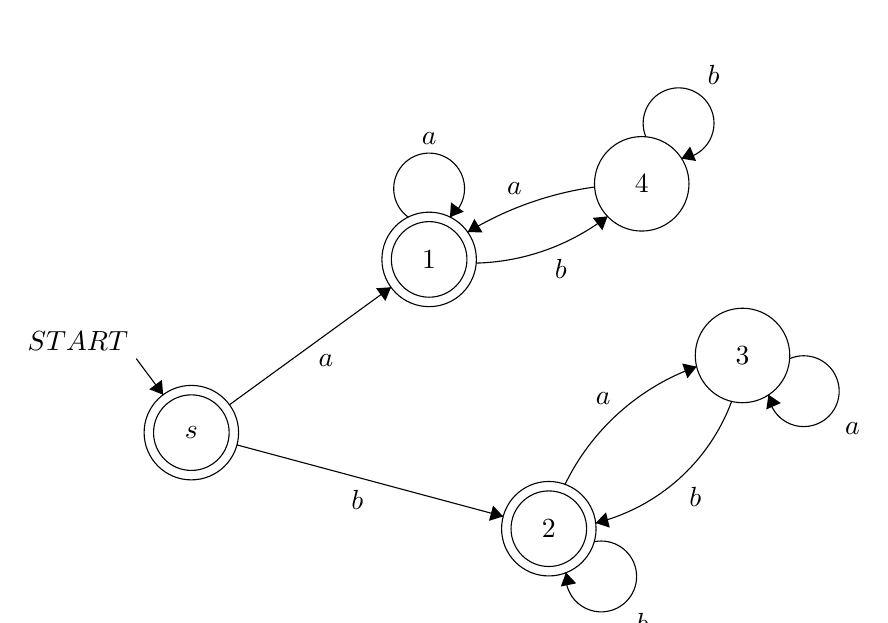
\begin{tikzpicture}[scale=0.2]
\tikzstyle{every node}+=[inner sep=0pt]
\draw [black] (12.7,-27.8) circle (3);
\draw (12.7,-27.8) node {$s$};
\draw [black] (12.7,-27.8) circle (2.4);
\draw [black] (27.8,-16.8) circle (3);
\draw (27.8,-16.8) node {$1$};
\draw [black] (27.8,-16.8) circle (2.4);
\draw [black] (35.4,-33.9) circle (3);
\draw (35.4,-33.9) node {$2$};
\draw [black] (35.4,-33.9) circle (2.4);
\draw [black] (47.7,-22.9) circle (3);
\draw (47.7,-22.9) node {$3$};
\draw [black] (41.3,-12) circle (3);
\draw (41.3,-12) node {$4$};
\draw [black] (15.12,-26.03) -- (25.38,-18.57);
\fill [black] (25.38,-18.57) -- (24.43,-18.63) -- (25.02,-19.44);
\draw (21.25,-22.8) node [below] {$a$};
\draw [black] (26.477,-14.12) arc (234:-54:2.25);
\draw (27.8,-9.55) node [above] {$a$};
\fill [black] (29.12,-14.12) -- (30,-13.77) -- (29.19,-13.18);
\draw [black] (38.271,-34.729) arc (101.62126:-186.37874:2.25);
\draw (40.92,-39.91) node [right] {$b$};
\fill [black] (36.49,-36.68) -- (36.16,-37.57) -- (37.14,-37.37);
\draw [black] (15.6,-28.58) -- (32.5,-33.12);
\fill [black] (32.5,-33.12) -- (31.86,-32.43) -- (31.6,-33.4);
\draw (23.24,-31.42) node [below] {$b$};
\draw [black] (9.2,-23.1) -- (10.91,-25.39);
\draw (5.5,-22.6) node [above] {$START$};
\fill [black] (10.91,-25.39) -- (10.83,-24.45) -- (10.03,-25.05);
\draw [black] (36.429,-31.087) arc (154.10136:109.51174:14.785);
\fill [black] (44.79,-23.61) -- (43.87,-23.41) -- (44.2,-24.35);
\draw (38.86,-26.04) node [above] {$a$};
\draw [black] (50.681,-23.108) arc (113.74356:-174.25644:2.25);
\draw (54.18,-27.54) node [right] {$a$};
\fill [black] (49.35,-25.39) -- (49.21,-26.33) -- (50.13,-25.92);
\draw [black] (39.133,-14.067) arc (-52.37:-88.48375:14.292);
\fill [black] (39.13,-14.07) -- (38.19,-14.16) -- (38.8,-14.95);
\draw (36.16,-16.74) node [below] {$b$};
\draw [black] (41.564,-9.023) arc (202.67131:-85.32869:2.25);
\draw (45.86,-5.73) node [above] {$b$};
\fill [black] (43.82,-10.4) -- (44.75,-10.55) -- (44.37,-9.63);
\draw [black] (30.247,-15.069) arc (121.21507:97.93118:21.201);
\fill [black] (30.25,-15.07) -- (31.19,-15.08) -- (30.67,-14.23);
\draw (33.21,-12.7) node [above] {$a$};
\draw [black] (47.009,-25.812) arc (-20.28933:-76.09757:12.382);
\fill [black] (38.37,-33.54) -- (39.27,-33.83) -- (39.03,-32.86);
\draw (44.71,-31.24) node [below] {$b$};
\end{tikzpicture}
\end{center}

First we should notice that the difference between ${|w|}_{ab}$ and ${|w|}_{ba}$ is at most $1$.
Because $s\in F$, $\epsilon \in L(A)$. Additionally, $s \mapsto_A^{a^*} q_1$ and $s \mapsto_A^{b^*} q_2$ makes $L(A)$ accept $a^*$ and $b^*$ since $q_1, q_2 \in F$.\\
Now we assume for a string $w$ for which $w \in L_2 \land  0 < |w| \le n$, $A$ accepts $w$. Then, we prove the same holds for $w'$ that $w' \in L_2 \land |w'| = n + 1$.\\
For $w'=v\sigma$, $A$ can distinguish the string $v,  (|v| \ge 1)$. \\
\begin{itemize}
	\item If $A$ accepts $v$, $A$ would be at state either $q_1$ or $q_2$.
	\begin{itemize}
		\item If $A$ is at state $q_1$ after reading $v$, the last symbol of $v$ is $a$. 
		\begin{itemize}
			\item If $\sigma$ is $a$, $w'$ has the same ocurrence of $ab, ba$ with $v$, so $w'\in L_2$. Since $A$ terminates in $q_1$ after reading $w'$, $w'\in L(A)$ too.
			\item If $\sigma$ is $b$, $w'$ has one more occurrence of $ab$ than $v$, so $ab$ occurs one more time than $ba$ in $w'$ and thus $w'\notin L_2$. Since $A$ terminates in $q_4$ after reading $w'$, $w' \notin L(A)$ too.
		\end{itemize}
		\item If $A$ is at state $q_2$ after reading $v$, the last symbol of $v$ is $b$. 
		\begin{itemize}
			\item If $\sigma$ is $b$, $w'$ has the same ocurrence of $ab, ba$ with $v$, so $w'\in L_2$. Since $A$ terminates in $q_2$ after reading $w'$, $w'\in L(A)$ too.
			\item If $\sigma$ is $a$, $w'$ has one more occurrence of $ba$ than $v$, so $ba$ occurs one more time than $ab$ in $w'$ and thus $w'\notin L_2$. Since $A$ terminates in $q_3$ after reading $w'$, $w' \notin L(A)$ too.
		\end{itemize}
	\end{itemize}
	\item If $A$ does not accept $v$, $A$ would be at state either $q_4$ or $q_3$.
	\begin{itemize}
		\item If $A$ is at state $q_4$ after reading $v$, the last symbol of $v$ is $b$. 
		\begin{itemize}
			\item If $\sigma$ is $a$, $w'$ has one more occurrence of $ba$ than $v$, so $ba$ occurs the same times as $ab$ in $w'$ and thus $w'\in L_2$. Since $A$ terminates in $q_1$ after reading $w'$, $w'\in L(A)$ too.
			\item If $\sigma$ is $b$, $w'$ has the same ocurrence of $ab, ba$ with $v$, so $w'\notin L_2$. Since $A$ terminates in $q_4$ after reading $w'$, $w' \notin L(A)$ too.
		\end{itemize}
		\item If $A$ is at state $q_3$ after reading $v$, the last symbol of $v$ is $a$. 
		\begin{itemize}
			\item If $\sigma$ is $b$, $w'$ has one more occurrence of $ab$ than $v$, so $ab$ occurs the same times as $ba$ in $w'$ and thus $w'\in L_2$. Since $A$ terminates in $q_2$ after reading $w'$, $w'\in L(A)$ too.
			\item If $\sigma$ is $a$, $w'$ has the same ocurrence of $ab, ba$ with $v$, so $w'\notin L_2$. Since $A$ terminates in $q_3$ after reading $w'$, $w' \notin L(A)$ too.
		\end{itemize}
	\end{itemize}
\end{itemize}
There we proved $L(A)=L_2$ for any length of string $w \in L_2$.

\end{enumerate}
\end{enumerate}
\label{lastpage}
\end{document}
